\chapter{Networking and mesh coordination}
\label{chap:rete}

\section{Network policies and reachability boundaries}

The trust zones of \autoref{fig:trust-zones} describe who can contact whom. The reachability boundaries
that derive from them are enforced by a network policy that Network-Manager publishes on Headscale.

Every node of the mesh network, be it a service or a user's device, carries one or more labels
called tags. The reachability rules are written on tags rather than on IP addresses, so as to
survive a change of a service's address, for example because it restarts on a different node.

Network-Manager collects all the rules into a single document and delivers it to Headscale only once,
at startup \cite{ramusb-code-acl-policy}.

Headscale in turn translates it into a packet filter: it tells every node that joins the network only about the
peers that the rules allow it to contact, and then sends it the subsequent updates concerning those peers.
In this way, a service that by policy must not contact another one is not even able to
see it in the network.

The rules, moreover, name only the party that opens the connection, so replies travel without a rule
in the opposite direction. In this way, for example, Security-Switch can contact Database-Vault, and the latter
can reply to the request, but is not able to initiate communication with it.

\section{Access grant lifecycle}

The two rules that concern the user are shown in \autoref{lst:acl-utente}. The tag
\texttt{TagStorageAccess} is temporary and is assigned at login; \texttt{TagMeshMember} is permanent and
is assigned when the device joins the network.

\Needspace{12\baselineskip}
\begin{lstlisting}[caption={The two rules that delimit the user's zones, from \texttt{policy.go}
\cite{ramusb-code-acl-policy}, with added comments.}, label={lst:acl-utente}]
{ // only an authenticated user, and Database-Vault, reach Storage-Service
    Action: "accept",
    Src:    []string{TagStorageAccess, TagDatabaseVault},
    Dst:    []string{dstAny(TagStorageService)},
},
{ // every registered user reaches Entry-Hub
    Action: "accept",
    Src:    []string{TagMeshMember},
    Dst:    []string{dstAny(TagEntryHub)},
},
\end{lstlisting}

At registration, Network-Manager creates for the new user an identity on Headscale and a pre-auth key,
that is, a single-use credential with which the device presents itself to the coordinator to join the network
\cite{ramusb-code-mesh-user}. The key is valid for fifteen minutes, and travels back up the chain of services to
the user inside the registration response.

The key is created already associated with the membership-only tag. The device that uses it therefore joins the
network and gains reachability to Entry-Hub's private network interface.

At login Network-Manager looks up the user's node and adds the second tag to it, then records an expiry
twelve hours from that moment \cite{ramusb-code-grant}.

Looking up the user's node, however, requires Network-Manager to keep a small SQLite database
containing the numeric identifier of the pre-auth key bound to the hash of the user's email, with the
schema shown in \autoref{lst:meshusers-schema}.

\Needspace{8\baselineskip}
\begin{lstlisting}[language=sql, caption={Schema of the email-to-pre-auth-key mapping table, from
\texttt{meshusers.go} \cite{ramusb-code-meshusers-schema}.}, label={lst:meshusers-schema}]
CREATE TABLE IF NOT EXISTS mesh_users (
	email_hash       TEXT PRIMARY KEY,
	pre_auth_key_id  INTEGER NOT NULL
);
\end{lstlisting}

The tag expiries are also persisted in the database, to prevent a restart of the service from turning
a twelve-hour grant into a perpetual grant. The schema of the table that holds them is shown in
\autoref{lst:grants-schema}.

\Needspace{10\baselineskip}
\begin{lstlisting}[language=sql, caption={Schema of the access grant table, from \texttt{store.go}
\cite{ramusb-code-grants-schema}.}, label={lst:grants-schema}]
CREATE TABLE IF NOT EXISTS grants (
	email_hash TEXT PRIMARY KEY,
	node_id    INTEGER NOT NULL,
	tag        TEXT NOT NULL,
	expires_at INTEGER NOT NULL
);
\end{lstlisting}

A periodic process, every five minutes, looks for expiries that have passed and revokes the expired grants
\cite{ramusb-code-sweep}. The row is deleted from the database before calling Headscale to remove
the tag, and the deletion is conditional on the exact expiry just read.
If in the meantime a login has renewed the grant, the expiry in the table no longer matches, so the deletion
touches no row and the sweep stops without contacting Headscale.
Calling Headscale first and deleting afterward would instead have risked also deleting the row
just rewritten by the concurrent login, taking away from the user a grant that had just been given.

\autoref{fig:acl-grant} summarizes the states that a user's node goes through.

\begin{figure}[H]
    \centering
    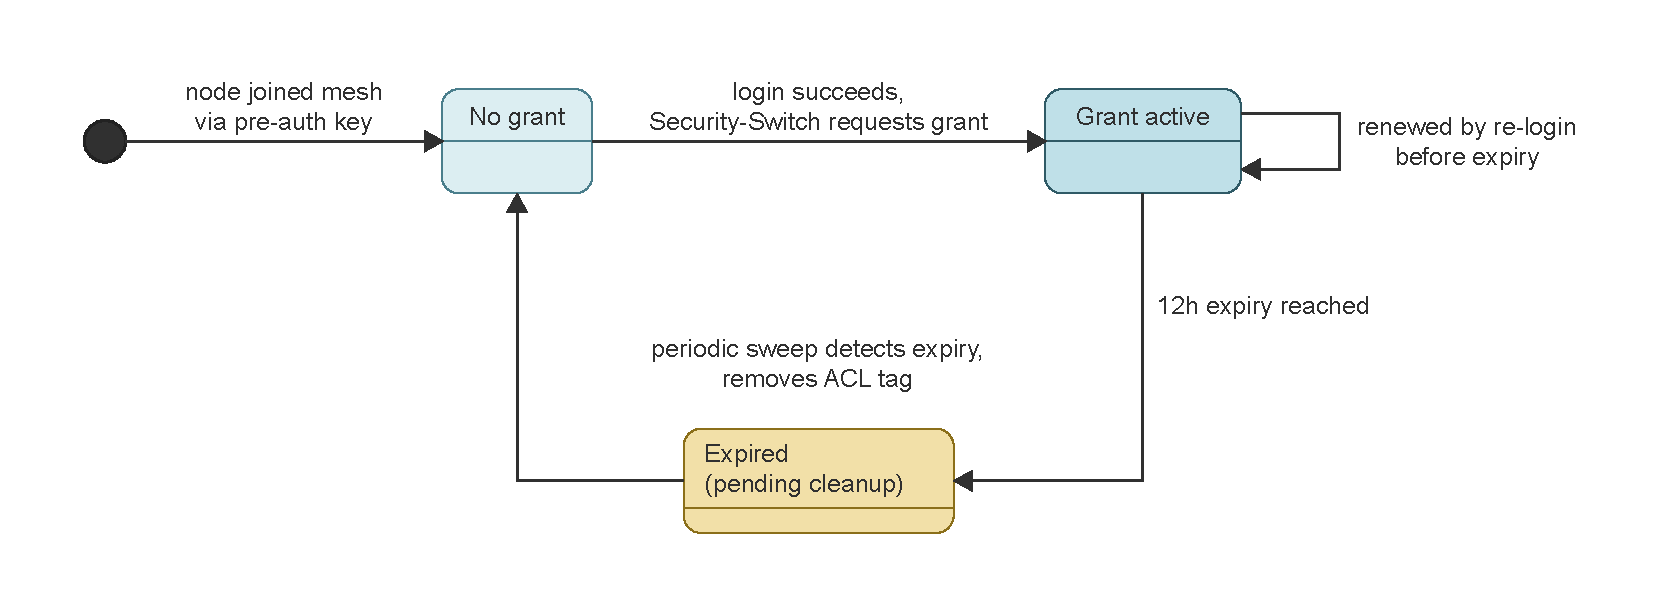
\includegraphics[width=\textwidth]{figures/10-operations-state-acl-grant.pdf}
    \caption{Lifecycle of the access grant associated with a user's node.}
    \label{fig:acl-grant}
\end{figure}

\section{The coordinator paradox: Headscale as a standalone service}
\label{sec:paradosso-coordinatore}

The Headscale documentation states that running Headscale on a machine that
belongs to the coordinated network is not recommended, because it can cause problems with name resolution through MagicDNS
\cite{headscale-faq}.

The coordinator must therefore remain outside the network it coordinates, and three consequences follow from this.

The first is that it cannot share a virtual machine or a container with any other component,
because all the others are members of the mesh.

The second is that the traffic with which Network-Manager creates the keys and assigns the tags cannot be
protected by its placement in the network, as is the case for every other internal call. It is the only
call between components of the system that crosses the public network, and the only one whose protection depends
entirely on mTLS and on the Headscale API key.

The third is that the coordinator must be publicly reachable, because a device that has not
yet joined the network must be able to contact it the first time in order to join the network.

Headscale, however, has a limitation that is relevant for RAM-USB: it offers no way to separate the coordination
protocol, which must be reachable by everyone, from the administrative API, which must be reachable only by
Network-Manager.
The separation was entrusted to a reverse proxy, which distinguishes the two surfaces based on the path
of the request \cite{ramusb-code-headscale-proxy}. Coordination requests pass without any check,
while administrative ones are accepted only if accompanied by a certificate issued by the
private Certificate-Authority, in addition to an API key that Headscale itself
requires. The administrative traffic is defended by two independent credentials because it is one of the most
sensitive surfaces.

The certificate presented by the proxy is instead issued by a public CA, for the same reason that
Entry-Hub's is.

\section{CG-NAT and the need for a dedicated public endpoint}

The central pool of not-yet-assigned IPv4 addresses was exhausted in 2011 \cite{icann-ipv4-2011}, and
to keep connecting new customers many Internet Service Providers have several subscribers share a single
public IPv4 address. The home router no longer receives a public address, but one
from the \texttt{100.64.0.0/10} block, valid only inside the operator's network and not
routable on the internet \cite{rfc6598}; it is a NAT managed by the operator that translates it into the shared
public address. This type of NAT is called Carrier-Grade NAT \cite{rfc6888}.
Since that NAT is not under the customer's control, the customer cannot open inbound ports on it
by themselves, and in general a server hosted at home is not reachable from the internet \cite{rfc6269}.
RAM-USB is designed so that it can also be hosted by home users, who therefore might not
have neither a public IPv4 address nor IPv6 connectivity. For this reason Headscale and Entry-Hub each reside on
their own Virtual Private Server, separate from the rest of the system. \autoref{chap:deployment} describes the actual placement of each component.
